\chapter{MXNet}
\section{Optimizing Memory Consumption in DL}
Over the last ten years, a constant trend in deep learning is towards deeper and larger networks. Despite rapid advances in hardware performance, cutting-edge deep learning models continue to push the limits of GPU RAM. So even today, it’s always desirable to find ways to train larger models while consuming less memory. Doing so enables us to train faster, using larger batch sizes, and consequently achieving a higher GPU utilization rate.

\subsection{Computation Graph}
A computation graph describes the (data flow) dependencies between the operations in the deep network. The operations performed in the graph can be either fine-grained or coarse-grained.

The concept of a computation graph is explicitly encoded in packages like Theano and CGT. In other libraries, computation graphs appear implicitly as network configuration files. The major difference in these libraries comes down to how they calculate gradients. There are mainly two ways: performing back-propagation on the same graph or explicitly representing a backwards path to calculate the required gradients.

\begin{figure}[!hbtp]
\centering
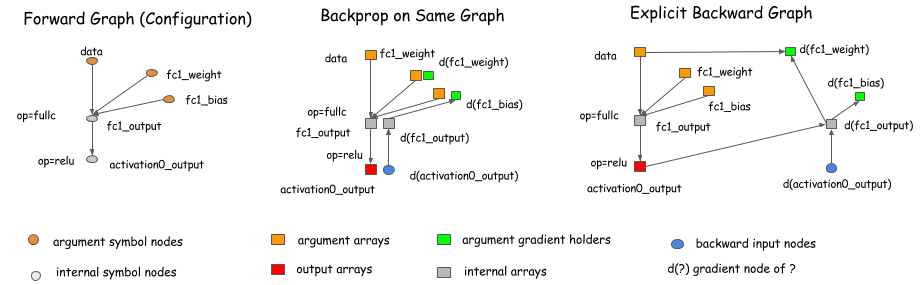
\includegraphics[width=0.85\textwidth]{MXNet/back_graph}
\caption{The implicitly \& explicitly back-propagation on Graph}
\end{figure}

Libraries like Caffe, CXXNet, and Torch take the former approach, performing back-prop on the original graph. Libraries like Theano and CGT take the latter approach, explicitly representing the backward path. In this discussion, we adopt the explicit backward path approach because it has several advantages for optimization.

We adopt the explicit backward path approach because it has several advantages for optimization.

Why is explicit backward path better? Two reasons:
\begin{itemize}
\item The explicit backward path clearly describes the dependency between computations.\\
Like the following case, where we want to get the gradient of \textbf{A} and \textbf{B}. As we can see clearly from the graph, the computation of the $d(C)$ gradient doesn’t depend on $F$. This means that we can free the memory of $F$ right after the forward computation is done. Similarly, the memory of $F$ can be recycled.
\begin{figure}[!hbtp]
\centering
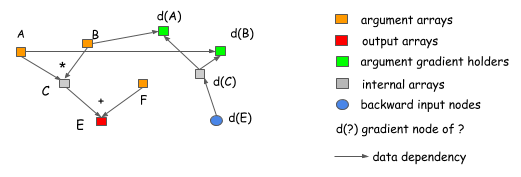
\includegraphics[width=0.85\textwidth]{MXNet/back_dep_prune}
\caption{Dependencies can be found quickly.}
\end{figure}

\item Another advantage of the explicit backward path is the ability to have a different backward path, instead of a mirror of forward one.\\
A common example is the split connectioncase, as shown in the following figure.
\begin{figure}[!hbtp]
\centering
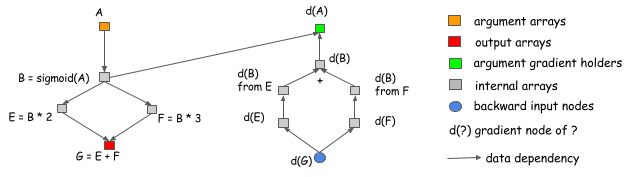
\includegraphics[width=0.85\textwidth]{MXNet/back_agg_grad}
\caption{Different backward path from forward path.}
\end{figure}
In this example, the output of \textbf{B} is referenced by two operations. If we want to do the gradient calculation in the same network, we need to introduce an explicit split layer. This means we need to do the split for the forward pass, too. In this figure, the forward pass doesn’t contain a split layer, but the graph will automatically insert a gradient aggregation node before passing the gradient back to \textbf{B}. This helps us to save the memory cost of allocating the output of the split layer, and the operation cost of replicating the data in the forward pass.
\end{itemize}

\subsection{What Can be Optimized?}
As you can see, the computation graph is a useful way to discuss memory allocation optimization techniques. Already, we’ve shown how you can save some memory by using the explicit backward graph. Now let’s explore further optimizations, and see how we might determine reasonable baselines for benchmarking.

Assume that we want to build a neural network with \textit{n} layers. Typically, when implementing a neural network, we need to allocate node space for both the output of each layer and the gradient values used during back-propagation. This means we need roughly $2n$ memory cells. We face the same requirement when using the explicit backward graph approach because the number of nodes in a backward pass is roughly the same as in a forward pass.

\subsubsection{In-place Operations}
One of the simplest techniques we can employ is \textit{In-place memory sharing} across operations. For neural networks, we can usually apply this technique for the operations corresponding to activation functions. 

''In-place'' means using same memory for input and output. But you should be careful about that the result is used by more than one operation! 

\subsubsection{Standard Memory Sharing}
In-place operations are not the only places where we can share memory. In the following example, because the value of B is no longer needed after we compute E, we can reuse B’s memory to hold the result of E.
\begin{figure}[!hbtp]
\centering
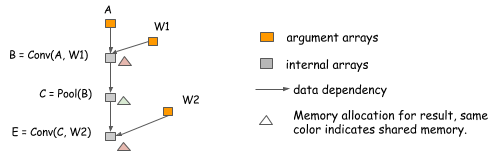
\includegraphics[width=0.85\textwidth]{MXNet/alloc_normal}
\caption{Standard Memory sharing between \textbf{B} \& the result of \textbf{E}.}
\end{figure}

Memory sharing doesn't necessarily require the same data shape. Note that in the preceding example, the shapes of \textbf{B} and \textbf{E} can differ. To handle such a situation, we can allocate a memory region of size equal to the maximum of that required by \textbf{B} and \textbf{E} and share it between them.

\subsection{Memory Allocation Algorithm}
Based on the '' In-Place Operatioins'', how can we allocate memory correctly?

The key problem is that we need to place resources so that they don’t conflict with each other. More specifically, each variable has a \textbf{life time} between the time it gets computed until the last time it is used. In the case of the multi-layer perceptron, the life time of \textit{fc1} ends after \textit{act1} get computed.
\index{Life Time}
See below figure:
\begin{figure}[!hbtp]
\centering
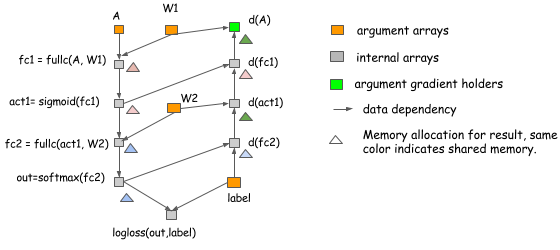
\includegraphics[width=0.85\textwidth]{MXNet/alloc_mlp}
\caption{Standard Memory sharing between \textbf{B} \& the result of \textbf{E}.}
\end{figure}

The principle is to allow memory sharing only between variables whose lifetimes don’t overlap. There are multiple ways to do this. You can construct the conflicting graph with each variable as a node and link the edge between variables with overlapping lifespans, and then run a graph-coloring algorithm. This likely has $O(n^2)$ complexity, where \textit{n} is the number of nodes in the graph. This might be too costly.

Let’s consider another simple heuristic. The idea is to simulate the procedure of traversing the graph, and keep a count of future operations that depends on the node.
\begin{figure}[!hbtp]
\centering
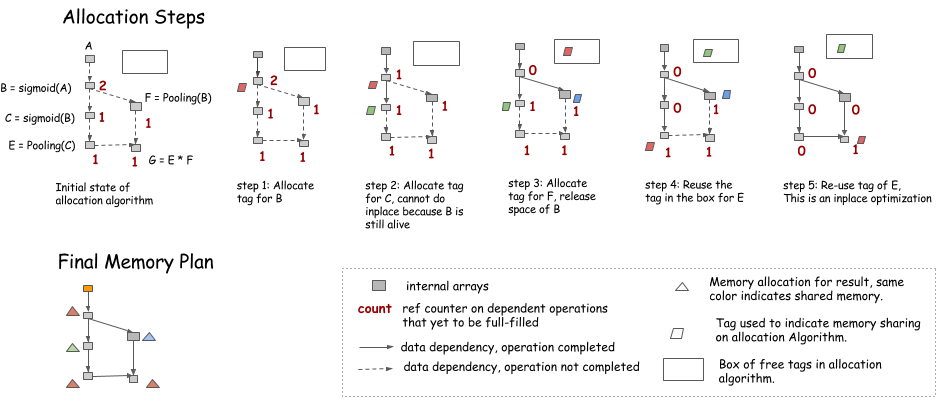
\includegraphics[width=0.95\textwidth]{MXNet/alloc_step}
\caption{Standard Memory sharing between \textbf{B} \& the result of \textbf{E}.}
\end{figure}
\begin{itemize}
\item An in-place optimization can be performed when only the current operation depends on the source (i.e. count == 1).
\item Memory can be recycled into the box on the upper right corner when the \textit{count} goes to 0.
\item When we need new memory, we can either get it from the box or allocate a new one. 
\end{itemize}

\textbf{Noet:} During the simulation, no memory is allocated. Instead, we keep a record of how much memory each node needs, and allocate the maximum of the shared parts in the final memory plan.

\subsection{Static vs. Dynamic Allocation}
The major difference is that static allocation is only done once, so we can afford to use more complicated algorithms. For example, we can search for memory sizes that are similar to the required memory block. The Allocation can also be made graph aware. We’ll talk about that in the next section. Dynamic allocation puts more pressure on fast memory allocation and garbage collection.

There is also one takeaway for users who want to rely on dynamic memory allocations: do not unnecessarily reference objects. For example, if we organize all of the nodes in a list and store then in a Net object, these nodes will never get dereferenced, and we gain no space. Unfortunately, this is a common way to organize code.

\subsection{Memory Allocation for Parallel Operations}
In the previous section, we discussed how we can simulate running the procedure for a computation graph to get a static allocation plan. However, optimizing for parallel computation presents other challenges because resource sharing and parallelization are on the two ends of a balance. Let’s look at the following two allocation plans for the same graph:
\begin{figure}[!hbtp]
\centering
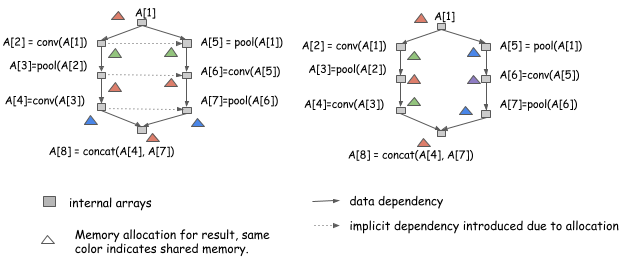
\includegraphics[width=0.95\textwidth]{MXNet/parallel_alloc}
\caption{Standard Memory sharing between \textbf{B} \& the result of \textbf{E}.}
\end{figure}

Both allocation plans are valid if we run the computation serially, {\bfseries from $A[1]$ to $A[8]$. } However, the allocation plan on the left introduces additional dependencies, which means we can't run computation of $A[2]$ and $A[5]$ in parallel. The plan on the right can. To parallelize computation, we need to take greater care. 

\subsubsection{Be Correct and Safe First}
Being correct is our first principle. This means to execute in a way that takes implicit dependency memory sharing into consideration. You can do this by adding the implicit dependency edge to the execution graph. Or, even simpler, if the execution engine is mutation aware, as described in \href{https://mxnet.incubator.apache.org/architecture/note_engine.html}{our discussion of dependency engine design}, push the operation in sequence and write to the same variable tag that represents the same memory region.

Always produce a safe memory allocation plan. This means never allocate the same memory to nodes that can be parallelized. This might not be ideal when memory reduction is more desirable, and we don’t gain too much when we can get benefit from multiple computing streams simultaneously executing on the same GPU.

\subsubsection{Try to Allow More Parallelization}
Now we can safely perform some optimizations. The general idea is to try and encourage memory sharing between nodes that can’t be parallelized. You can do this by creating an ancestor relationship graph and querying it during allocation, which costs approximately $O(n^2)$ in time to construct. We can also use a heuristic here, 
for example, color the path in the graph. As shown in the following figure, when you try to find the longest paths in the graph, color them the same color and continue.
\begin{figure}[!hbtp]
\centering
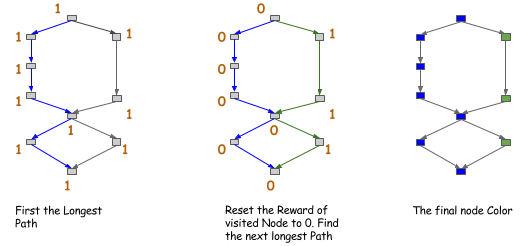
\includegraphics[width=0.95\textwidth]{MXNet/graph_color}
\caption{Color the longest paths in the Graph.}
\end{figure}

After you get the color of the node, you allow sharing (or encourage sharing) only between nodes of the same color. This is a stricter version of the ancestor relationship, but is costs only $O(n)$ of time if you search for only the first $k$ path.

\subsection{How Much Can we Save ?}
On coarse-grained operation graphs that are already optimized for big operations, you can reduce memory consumption roughly by half. You can reduce memory usage even more if you are optimizing a fine-grained computation network used by symbolic libraries, such as Theano.

\subsection{References}
More details can be found in: \href{https://mxnet.incubator.apache.org/architecture/note_memory.html#how-much-can-you-save}{Opimizing the Memory Consumption in DL(MXNet)}.


\section{Deep Learning Programming Style}

Two of the most important high-level design decisions

\begin{itemize}
\item Whether to embrace the symbolic or imperative paradigm for mathematical computation

\item Whether to build networks with bigger or more atomic operations
\end{itemize}

\subsection{Symbolic vs. Imperative Program}

即:符号式编程 vs. 命令式编程

Symbolic programs are a bit different. With symbolic-style programs, we first define a (potentially complex) function abstractly. When defining the function, no actual numerical computation takes place. We define the abstract function in terms of \textbf{placeholder values}(占位符). Then we can compile the function, and evaluate it given real inputs. 

This operation generates a computation graph (also called a symbolic graph) that represents the computation.

Most symbolic-style programs contain, either explicitly or implicitly, a compile step. 

真正的计算只发生在传入数值之时,在这之前,都没有任何计算发生。

The defining characteristic of symbolic programs is their clear separation between building the computation graph and executing it.For neural networks, we typically define the entire model as a single compute graph.

\subsection{Imperative Programs Tend to be More Flexible}

未完待续...




